\documentclass[class=article,border=5pt,tikz]{standalone}
\usepackage{xfrac}% \sfrac

\begin{document}
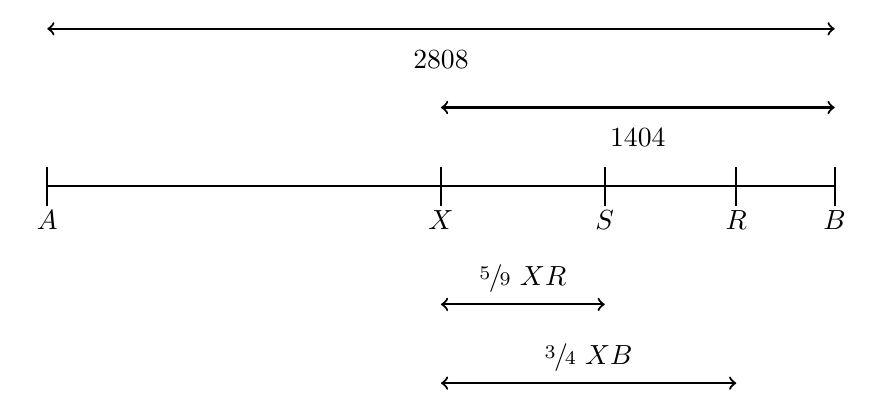
\begin{tikzpicture}[thick, scale=10]
    % coordinates to be reused
    \coordinate (A) at (0,0);
    \coordinate (X) at (0.5,0);
    \coordinate (S) at (0.708,0);
    \coordinate (R) at (0.875,0);
    \coordinate (B) at (1,0);
    % draw lines with labels
    \draw (A) node [below,yshift={-5pt}] {$A$}
       -- (X) node [below,yshift={-5pt}] {$X$}
       -- (S) node [below,yshift={-5pt}] {$S$}
       -- (R) node [below,yshift={-5pt}] {$R$}
       -- (B) node [below,yshift={-5pt}] {$B$} ;
    % add tickmarks
    \draw (0,-0.025) -- (0,0.025);
    \draw (0.5,-0.025) -- (0.5,0.025);
    \draw (0.708,-0.025) -- (0.708,0.025);
    \draw (0.875,-0.025) -- (0.875,0.025);
    \draw (1,-0.025) -- (1,0.025);
    % add arrows
    \draw [<->] (0,0.2) -- (1,0.2) node[midway,above=-18pt]{2808}; 
    \draw [<->] (0.5,0.1) -- (1,0.1) node[midway,above=-18pt]{1404}; 
    \draw [<->] (0.5,-0.25) -- (0.875,-0.25) node[midway,below=-18pt]{$\sfrac{3}{4}~XB$}; 
    \draw [<->] (0.5,-0.15) -- (0.708,-0.15) node[midway,below=-18pt]{$\sfrac{5}{9}~XR$}; 
\end{tikzpicture}
\end{document}
